\documentclass[conference]{IEEEtran}
\usepackage[hidelinks]{hyperref}
\usepackage{graphicx}
\hypersetup{
    colorlinks=true,
    linkcolor=blue,
    filecolor=blue,
    urlcolor=blue
}
\begin{document}
\title{CSE342: Statistical Machine Learning Report}
\makeatletter
\newcommand{\linebreakand}{%
  \end{@IEEEauthorhalign}
  \hfill\mbox{}\par
  \mbox{}\hfill\begin{@IEEEauthorhalign}
}
\makeatother

\author{
    \IEEEauthorblockN{Prakhar Gupta}
  \IEEEauthorblockA{\texttt{Roll No. 2021550} \\
  \texttt{CSAI Dept.} \\
  \texttt{prakhar21550@iiitd.ac.in}}
    \and
    \IEEEauthorblockN{Shreyas Kabra}
    \IEEEauthorblockA{\texttt{Roll No. 2021563} \\
    \texttt{CSAI Dept.} \\
    \texttt{shreyas21563@iiitd.ac.in}}
}

\maketitle

\begin{abstract}
    This report presents a machine learning project completed for the course \textit{CSE 342: Statistical Machine Learning} at the \textit{Indraprastha Institute of Information Technology, New Delhi}. The project, a Kaggle competition, involved creating an accurate fruit classification model with 20 possible labels. 
    The report briefly describes the problem statement, the data set provided, and the different pre-processing steps taken to prepare the given data for analysis. It then outlines the various machine learning algorithms tested during the project, including the respective results, observations, and evaluation metrics. 
    The report concludes with a summary of the project and provides relevant references. Overall, the report serves as a comprehensive summary of the project, presenting the application of various machine learning algorithms.
\end{abstract}
\begin{IEEEkeywords}
    PCA, LDA, logistic regression, cross validation, hyperparameter tuning, agglomerative clustering, meanshift clustering, DBSCAN clustering.
\end{IEEEkeywords}

% Introduction section
\section{Introduction}
    The problem is a fruit classification problem where a fruit is to be classified into one of 20 class labels.
    The aim of the project was to build a machine learning model to classify a fruit into one of 20 fruit labels. The dataset consists of 1216 samples, where each is classified into any label. The dataset and the competition is hosted on Kaggle [1]. 

% Outlier detection section
\section{Outlier Detection}
    The data set was checked for outliers by implementing the \textit{Local Outlier Factor} algorithm. The hyperparameter for the number of neighbours in the \textit{Local Outlier Factor} was set to 4 after performing \textit{k-fold cross validation} on the training data set. 
    The algorithm found 3 outliers in the data set and the outliers were removed from the training data set. When the \textit{Local Outlier Factor} algorithm was implemented along with the other algorithms mentioned in this report, the validation accuracy of the model was found to increase from 85.5\% to 85.99\%. 

% Dimensionality reduction section
\section{Dimensionality Reduction}
    Dimensionality reduction is a crucial pre-processing step in machine learning. It is implemented to reduce the number of features while retaining the maximum amount of information. By reducing the number of features, the model is able to train faster and the model is less prone to overfitting. The following dimensionality reduction algorithms were implemented on the training data set to reduce the number of features-
% Principal component analysis subsection
\subsection{Principal Component Analysis}
    The large number of features in the data set made it critical to perform \textit{principal component analysis}[2][3] on the given data set to reduce the number of features. It is implemented to reduce the number of features while retaining the maximum amount of information. \textit{Elbow method} and \textit{k-fold cross validation} was implemented to determine the optimal number of principal components. \textit{Elbow method} determined the optimal number of components to be 91 components, however, that resulted in a poor accuracy of around 74\%. 
    The \textit{k-fold cross validation} found the optimal number of components to be around 417 components, which resulted in a better accuracy of about 80\%.
    Due to higher accuracy, the number of components was set to 417 for the rest of the project.
% Linear discriminant analysis subsection
\subsection{Linear Discriminant Analysis}
    \textit{Linear discriminant analysis}[4][5] was also performed on the data set to reduce the number of features. It is implemented to maximize the separation between the classes. The range of the number of components for the project was 1 to 19 since the data set had 20 classes. \textit{Elbow method} and \textit{k-fold cross validation} was implemented to determine the optimal number of principal components. \textit{Elbow method} determined the optimal number of components to be 16 components, however, that resulted in a poor accuracy of around 76\%. 
    The \textit{k-fold cross validation} found the optimal number of components to be around 19 components, which resulted in a better accuracy of about 81\%.
    Due to higher accuracy, the number of components was set to 19 for the rest of the project.

% Unsupervised clustering
\section{Unsupervised Clustering}
    Unsupervised clustering algorithms aim to create clusters for the sample points based on the training data set. Adding a cluster feature to the data set after performing unsupervised clustering algorithms identifies correlations between the sample data points, thus finding the trends and groupings in the dataset, which may help in the supervised classification of the data set. The following unsupervised clustering algorithms were implemented on the training data set to create unsupervised clusters- 
% Agglomerative clustering subsection
\subsection{Agglomerative Clustering}
    \textit{Agglomerative clustering}[6] algorithm was implemented on the data set to cluster the training data and appending the unsupervised cluster labels to the training data. The unsupervised cluster labels were used as a feature in the training data to identify patterns and groupings in the dataset, which would otherwise not be apparent. Grouping the similar data together was expected to improve the accuracy of the model. For implementing agglomerative clustering, the hyperparameter for the number of clusters was set to 4 after performing \textit{k-fold cross validation}[7] on the training data set. 
% DBSCAN clustering subsection
\subsection{DBSCAN Clustering}
    \textit{DBSCAN clustering}[8] algorithm was implemented on the data set to cluster the training data and appending the unsupervised cluster labels to the training data. The hyperparameters set for implementing \textit{DBSCAN clustering} were set by grid search and the hyperparameters were set to \textit{eps} = 0.5 and \textit{min\_samples} = 5.
% K-Means clustering subsection
\subsection{K-Means clustering}
    \textit{K-means clustering}[9] was used on the data set to cluster the data set and compute a new feature using unsupervised clustering. The hyperparameter for the number of clusters was set to 19 after performing \textit{k-fold cross validation} on the training data set. 
% Comparison of clustering algorithms
\\ Amongst \textit{agglomerative, DBSCAN, and k-means clustering}, \textit{agglomerative clustering} was found to be the most effective in improving the accuracy of the model and was used for the rest of the project.

% Logistic Regression
\section{Logistic Regression} 
    \textit{Logistic Regression}[10]  is a supervised classification algorithm implemented to classify data into two classes, which is called binary logistic classification. In this project, the \textit{One vs All} method was used to implement \textit{Logistic Regression} for the 20 class labels classification. Amongst other classification methods, \textit{Logistic Regression} was found to be the most effective in improving the accuracy of the model.

% Ensembling Methods
\section{Ensembling Methods}
    \textit{Ensembling methods} are used to combine the predictions of multiple models to improve the accuracy of the model. 
    The \textit{Voting classifier} ensembling method was implemented with \textit{Logistic Regression and DBSCAN clustering}, \textit{Logistic Regression and Agglomerative clustering}. The accuracy of the model fell from 85.5\% to close to 79\%, and hence, the ensembling methods were not perform for the creation of the model. 

%  References section
\section{References}
    [1] \href{https://www.kaggle.com/competitions/sml-project/overview}{Kaggle Competition} \\ \relax
    [2] \href{https://en.wikipedia.org/wiki/Principal_component_analysis}{Principal Component Analysis} \\ \relax
    [3] \href{https://scikit-learn.org/stable/modules/generated/sklearn.decomposition.PCA.html}{PCA in Scikit-learn} \\ \relax
    [4] \href{https://en.wikipedia.org/wiki/Linear_discriminant_analysis}{Linear Discriminant Analysis} \\ \relax
    [5] \href{https://scikit-learn.org/stable/modules/generated/sklearn.discriminant_analysis.LinearDiscriminantAnalysis.html}{LDA in Scikit-learn} 
    \\ \relax
    [6] \href{https://scikit-learn.org/stable/modules/generated/sklearn.cluster.AgglomerativeClustering.html}{Agglomerative Clustering} \\ \relax
    [7] \href{https://scikit-learn.org/stable/modules/generated/sklearn.model_selection.KFold.html}{K-Fold Cross Validation} \\ \relax
    [8] \href{https://scikit-learn.org/stable/modules/generated/sklearn.cluster.DBSCAN.html}{DBSCAN Clustering} \\ \relax
    [9] \href{https://scikit-learn.org/stable/modules/generated/sklearn.cluster.KMeans.html}{K-Means Clustering} \\ \relax
    [10] \href{https://scikit-learn.org/stable/modules/generated/sklearn.linear_model.LogisticRegression.html}{Logistic Regression} \\ \relax

% Figure of the model
\begin{figure}[htbp]
    \hbox{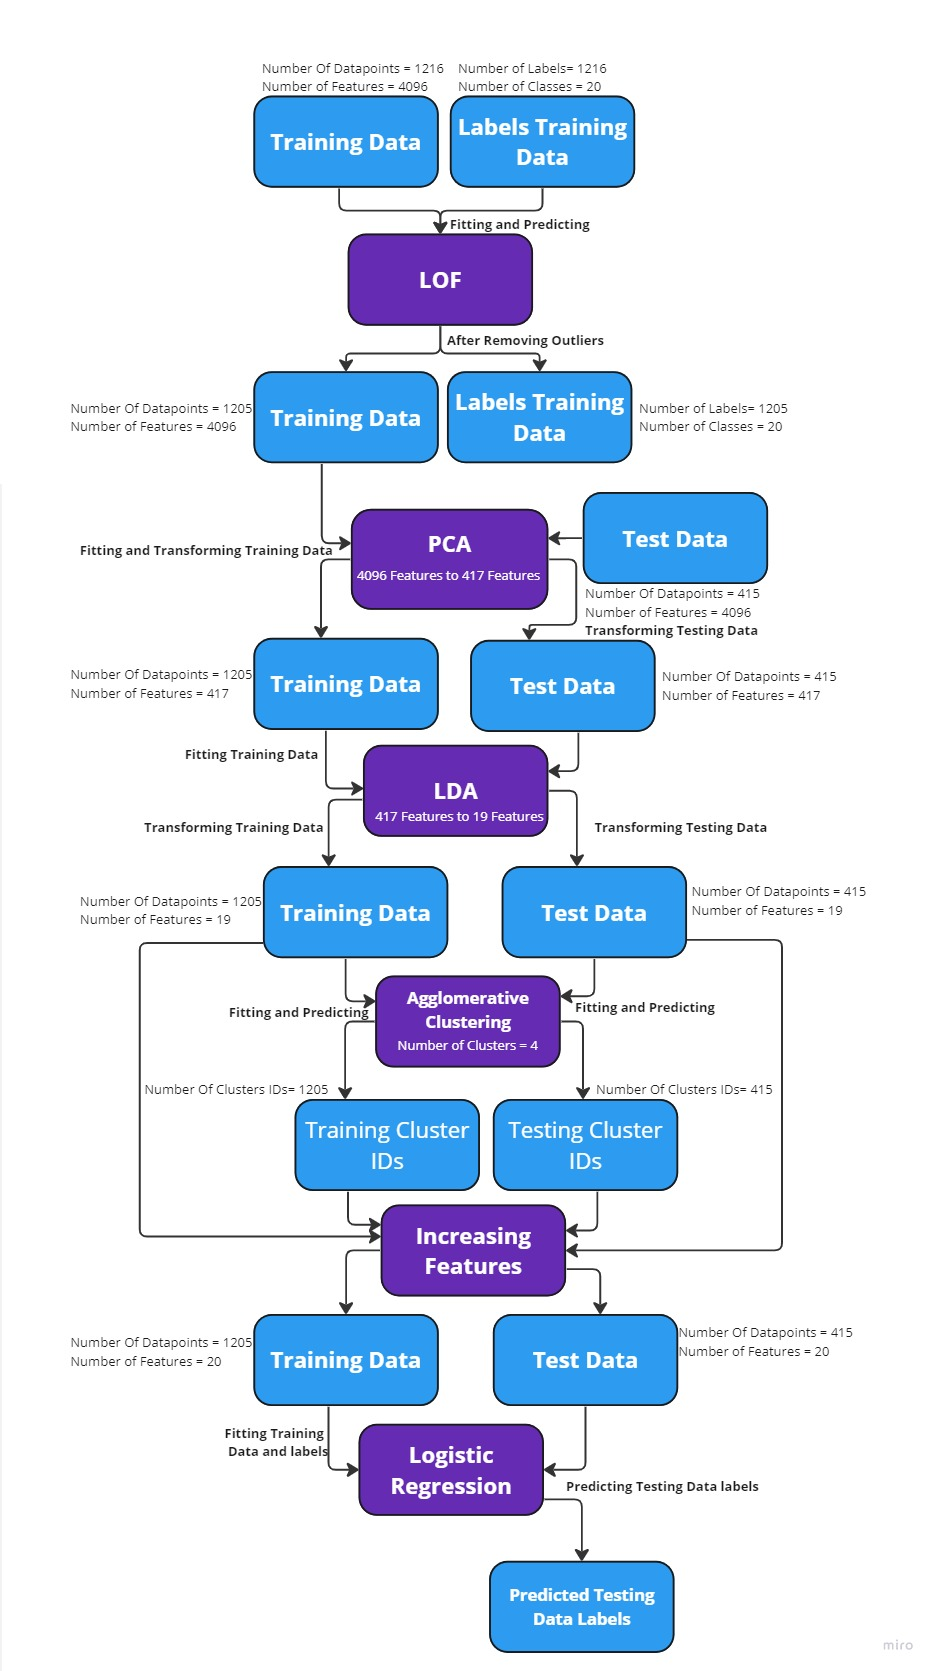
\includegraphics[width=1.3\columnwidth]{Diagram.jpg}}
    \caption{Figure for the model pipeline}
    \label{fig}
\end{figure}

\end{document}

